%\documentclass[acmjacm,acmnow]{acmtrans2m}
\documentclass[10pt,letterpaper]{article}

\usepackage{graphicx}
\usepackage{url}
\usepackage{color}
\usepackage{hyperref}

\newcommand{\projectnamefull}{\textit{Programming Abstractions for
    Large-Scale Distributed Applications} }

\newcommand{\upup}{\vspace*{-0.5em}}
\newcommand{\up}{\vspace*{-0.25em}}
\newcommand{\sagamapreduce }{SAGA-MapReduce }

\newcommand{\I}[1]{\textit{#1}}
\newcommand{\B}[1]{\textbf{#1}}
\newcommand{\T}[1]{\texttt{#1}}

\newcommand{\BI}[1]{\B{\I{#1}}}

% \ifpdf
%   \DeclareGraphicsExtensions{.pdf, .png, .jpg}
% \else
%   \DeclareGraphicsExtensions{.ps, .eps}
% \fi

\long\def\comment#1{{\bf \textcolor{magenta}{\bf #1}}}
\long\def\ccomment#1{{\bf \textcolor{blue}{\bf #1}}}
\newcommand{\C}{\comment}
\newcommand{\CC}{\ccomment}

\newcommand{\yes}{$\bullet$}

\newif\ifdraft
\drafttrue
\ifdraft
 \newcommand{\amnote}[1]{   {\textcolor{magenta} { ***Andre:    #1 }}}
 \newcommand{\hknote}[1]{ {\textcolor{blue}    { ***Hartmut:   #1 }}}
 \newcommand{\jhanote}[1]{  {\textcolor{red}     { ***Shantenu: #1 }}}
 \newcommand{\note}[1]{ {\textcolor{red}    { #1 }}}
\else
 \newcommand{\amnote}[1]{}
 \newcommand{\jhanote}[1]{}
 \newcommand{\hknote}[1]{}
 \newcommand{\note}[1]{}
\fi

% \markboth{Shantenu Jha et al}{Abstractions for Large-Scale Distributed
%   Applications and Systems}

\begin{document}

\title{SAGA: A Programming System for Distributed Applications} 

\begin{abstract}
  
  In the strictest sense, SAGA is the {\it Simple API for Grid Applications}. 
  For the purposes of this paper, we will refer to SAGA -- as a Programming
  System for Distributed Applications, and which consists of an implementation
  of the API, an core library and a set of adaptors which bind specific
  functionality to a specific middleware....
  As we will show, it is designed for a broad range of applications
  that aim to use a variety of distributed systems.
   
  A large number of applications motivated the design of SAGA.
  Admittedly these were applications that were
  first generation grid/distributed application, in that
  they were simple generalizations of legacy parallel/cluster
  applications.
  Notwithstanding, SAGA has been utilized to develop distributed
  applications that are significantly more complex and sophisticated
  (SAGA Montge, EnKF, Distributed Adaptive Replica Exchange)
  Software designed close to application, yet with sufficient
  degree of abstraction so as to enable broad uptake and general
  usability....

  Now say something about the implementation..
\end{abstract}

\maketitle

\begin{verbatim}

Scope of the CPC Paper

1.  Background: changing landscape of computational/digital
  infrastructure:
  - Traditional  Grids	+ Distributed Systems
  - Emerging Distributing Systems (Clouds, distributed data-store..)
  - High-end machines are becoming heterogenous, but at a different
        level of granularity
    Implication of the heterogenity of monolithic systems implies

  Develop scientific applications for all of the above -- in a
  "Standard"  uniform way. This is SAGA i.e, let us not just
  stay confined to traditional Grids. But we need to be very 
  clear that SAGA is applicable only for certain classes of 
  applications; SAGA != MPI; SAGA != a programming model per se
  and not an execution model (like MPI). SAGA supports
  different PM and ExecutionModels.

  Motivation: 
  Traditional Grid Systems:
    - heterogeneity (of what?)
    - .. 
  
   Emerging Distributed Systems:
    - heterogeneity (system interface, but also semantic difference)

   High-End Motivation:
     Why SAGA on these machines?

   SAGA provides the fundamental abstractions --- functionality,... ,
   that are required to develop applications in a system independent
   fashion
 
  Portability: syntactic, semantic and platform independence.

  SAGA Programming System:  (Engine + Packages) + Adaptors + Development tools for SAGA

  The API is exposed via the Engine (functional:context, session,
  non-functional:others) and Packages (functional and non-functional)


2. Some Distributed SCIENTIFIC Applications .. 
   possible use cases..

3. How these features/requirements are supported?
   Could have overlap with "requirements" 
   Develop "requirements"
   ....

4. All the Gory Details that have been developed to support the points
   in section 3.

   This is where OOPSLA paper comes in handy. Lots of the meat 
   is the same, but presented in a different perspective and style.

5. Applications that utilize these... and how.. for what.. (Broad spectrum)
   .. talk about N applications that we've developed
   .. show the specific features from Section 3 and how they are
   addressed/utilised/or contribute to the application usage
  
What is the contribution of this Paper: OOPSLA Paper is Implementation
paper + MCS Paper is Interface Paper, this is a mege of the two using
a consistent vocabulary along with applications.

\end{verbatim}
\newpage

\section{Introduction} {\bf SJ}

The process of developing and deploying large-scale distributed
applications presents a critical and challenging agenda for
researchers and developers working at the intersection of computer
science, computational science and a diverse range of application
areas. 

\note{Discuss briefly power of standards. Mention that C++ (our) Implementation follow standards. As does JAVA (Vrije). JSAGA; mostly independent complete implementations, but also implementations of convenience}

\section{Applications}\label{application}{\bf SJ }

\note{Introduce applications -- motivate SAGA}
\note{In this section we discuss a design philosophy of distributed applications}

\subsubsection*{Power of Abstractions}

\noindent \I{Distributed Applications and Tools:} SAGA has been used
to develop system-level tools and applications from each of the three
different types as shown in Fig 1(b): (i) Applications where local
functionality is swapped for distributed functionality, or where
distributed execution models are provided; (ii) Applications that are
developed using well known patterns, for example MapReduce, which in
turn is implemented using SAGA; (iii) Finally, applications based upon
frameworks that are developed using SAGA. These frameworks support
specific application-level and system functionality and can be used by
multiple applications (hence a framework and not an application-level
solution).  In this proposal we will discuss the latter two
categories; numerous examples of the first type can be found in papers
at ~\cite{saga_papers}.

\begin{figure}[!ht]
  \up\up
  \begin{center}
      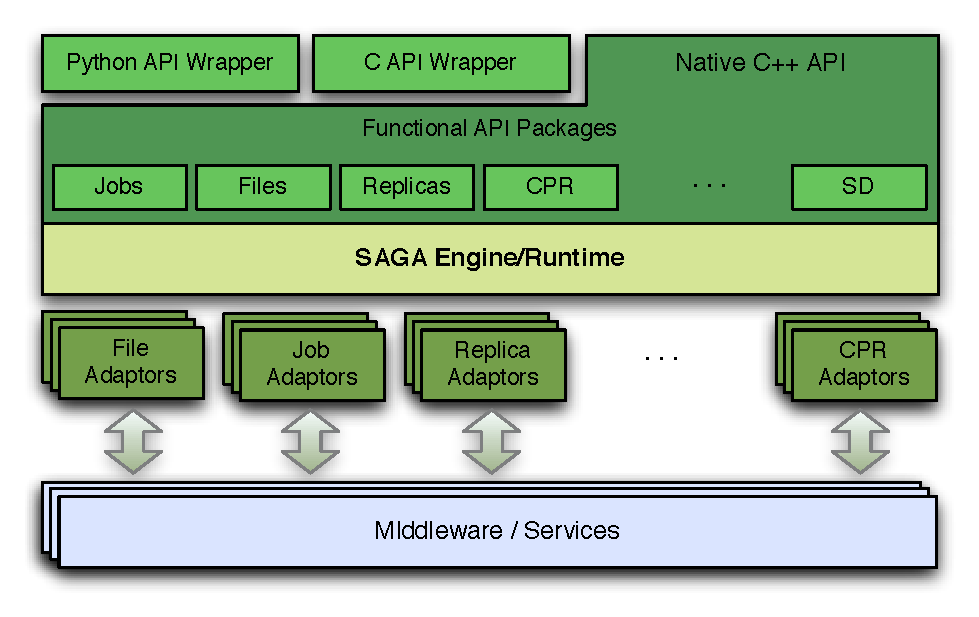
\includegraphics[width=0.45\textwidth]{../figures/stci_saga_figures-1.pdf}
      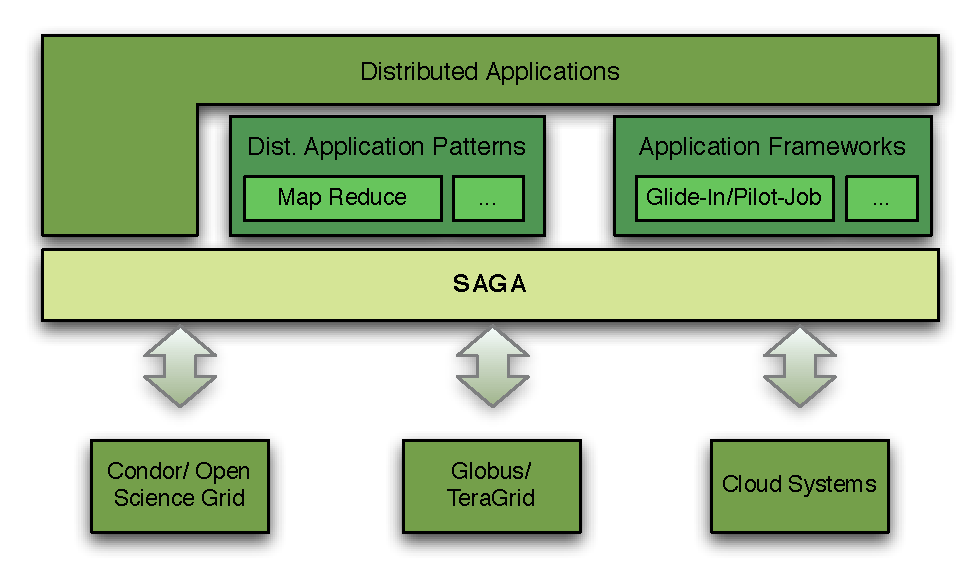
\includegraphics[width=0.48\textwidth]{../figures/stci_saga_figures.pdf}
  \end{center}
  \up\up\up\up\up\up\up\up\up\up
  \caption{\small (Left) Layered schematic of the different components
    of the SAGA landscape.  Middleware specific adaptors applications
    developed using SAGA make applications developed using SAGA grid
    portable. (Right) Schematic showing the different ways in which
    SAGA can be used to develop distributed applications}
 \label{sagalayer}
\end{figure}

\subsubsection*{Compute Intensive Applications}

We have developed a framework that facilitates the use of multiple heterogeneous resources for a range of applications. The framework is general purpose, and can overcome traditional limitations and can be used over a wide-range of production environments~\cite{saga_royalsoc}. Interestingly the same framework can be used to marshall different types and sizes of resources. For example the BigJob abstraction that we first employed on 512-node Linux Clusters can also be used for monolithic usage on Ranger -- a 64000 node machine~\cite{saga_iccs09}. It is also important to mention that the SAGA-based framework discussed is extensible, in that it can be used to implement many other application in addition to those it was initially developed for (molecular modelling). The power to do so arises from simple design decisions: the use of standard interfaces on the one hand, and the use of appropriate programmatic and system-level abstractions.

In a series of recent publications (Ref~\cite{saga_escience08}\cite{saga_royalsoc}\cite{saga_iccs09}), we have have shown how SAGA can be gradually used to develop the capabilities required by applications to effectively utilize heterogeneous infrastructure. As a first step, we demonstrated that the time-to-solution (i.e. wall-clock time) goes down as the number of resources increases.  It is important to note that for the end-user, the complexity of using one resource is the same as using multiple resources.  Initially in Ref~\cite{saga_escience08} we demonstrated a simple but effective coupling of SAGA with a molecular modelling package (NAMD) to create the basic infrastructure to establish the capability to utilize multiple distributed resources and a concomitant reduced time-to-solution.  Interestingly, this was possible in spite of the primitive infrastructure employed. In the second publication~\cite{saga_royalsoc} (three months later) we showed how we used SAGA to develop ``system-level'' abstractions (bigjob, manyjob) to enhance scalability and flexibility in resource utilization (and thus overcoming a specific performance bottleneck); the same system-level abstractions also eased application deployment and run-time management somewhat.  Finally, in Ref~\cite{saga_iccs09} (after a further two months) we showed how a framework that implements the abstractions when developed for one application was utilized by another application (Petroleum Engineering Application), and in general how it could be utilized for a large-class of applications (multiple loosely-coupled components).  In addition to distributed resources, the framework was shown to increase throughput and decrease time-to-solution on a single large machine (a 64,000 core machine at TACC) -- compared to the situation when the system-level abstractions were not used.  This incremental, modular but relatively speedy development provides testimony to the power of application and system-level abstractions and a general-purpose programming system that can support their development.

\note{Talk about Distributed Autonomic Applications..}

\subsubsection*{Data Intensive Applications for Grids and Clouds:}
MapReduce has emerged as a very successful and popular data-parallel
programming model. However, the question arises as to whether
MapReduce and other programming models for data-intensive computing
are viable independent of the underlying infrastructure?  What are the
limitations of the data-parallel programming model? To address these
questions, as well as to validate the abstractions that the SAGA
interface supports, we established in Ref~\cite{saga_ccgrid09}, that
the SAGA programming system provides a standard interface, that can
support simple, yet powerful programming models for data-intensive
applications.  Specifically, we implemented a simple data parallel
programming task (MapReduce) using SAGA; this involved the parallel
execution of simple, embarrassingly parallel data-analysis tasks.  We
demonstrated that the SAGA-based implementation is infrastructure
independent, whilst still providing control over the deployment,
distribution and run-time decomposition. We have written adaptors to
HDFS and to BigTable, thus providing the ability to use SAGA-based
MapReduce framework in native infrastructure as well.  We are now
developing applications (Genome Sequencing) that have not
traditionally been written using MapReduce, and are understanding
their performance.  This is an illustrative example of the kind of
empirical testing that is made possible using SAGA: one can build
infrastructure independent frameworks upon which applications can be
developed, tested and then improved upon. The ability to experiment
with the development of distributed applications and gain empirical
understanding of what works -- from infrastructure, to abstractions,
to specific optimizations, has been noticeable by its absence. SAGA
provides the ability to do so in a general purpose, extensible way --
possibly for the first time.

Although Clouds are a nascent infrastructure, there is a ground swell
of interest to adapt these emerging powerful infrastructure for
large-scale scientific applications. Inevitably, and as with any
emerging technology, the unified concept of a Cloud will evolve into
different flavors and implementations, with distinct underlying system
interfaces, semantics and infrastructure. 

% For example, the operating % environment of Amazon's Cloud (EC2) is very different from that of % Google's Cloud. Specifically for the latter, there already exist % multiple implementations of Google's Bigtable, such as HyberTable, % Cassandra and HBase. There is bound to be a continued proliferation of % such Cloud based infrastructure; this is reminiscent of the plethora % of Grid middleware distributions.  

A fundamental question at the heart of all these important considerations, is the question of how scientific applications can be developed so as to utilize as broad a range of distributed systems as possible, but with the flexibility and performance that large-scale scientific applications demand.  Having established the effectiveness of SAGA in Ref.~\cite{saga_ccgrid09}, the focus of Ref.~\cite{saga_interop09} was to use SAGA-based MapReduce as an exemplar to establish the interoperability aspects of the SAGA programming system.  Specifically, it demonstrated that \sagamapreduce is usable on traditional (Grids) and emerging (Clouds) distributed infrastructure {\it concurrently and cooperatively towards a solution of the same problem instance}.  It established how to use the {\it same} implementation of \sagamapreduce to solve the same instance of the word counting problem, by using different worker distributions over Clouds and Grid systems, and thereby also test for interoperability between different flavors of Clouds as well as between Clouds and Grids.


\section{An Overview of SAGA} {\bf AM}

{\it SAGA in a Nutshell}

\section{Design of the API} {\bf AM}

\section{SAGA Programming System} {\bf HK}

\subsection{Design Philosophy}

\note{A lot of the contact will be similar to the OOPSLA paper, however, we
will have to consistently i) make connections with ``principles of
distributed computing'', ii) make connections with our ``design
decisions'' and (not just objectives), express the tradeoffs and iii)
challenges..}

\note{Also discuss PIMPL..  and explain why (critical) it is required
for these (distributed) systems.. (hide implementation details - extensibility,
lightweight facade objects - well integrated with host language,
easy injection of engines functionality)}

\subsection{SAGA Engine}

\begin{itemize}
	\item sync, async, task
	\item asynchronous factories
	\item adaptor selection (adaptor registration, error handling and reporting,
	\item on call by call basis)
	\item tasks, task container
	\item bulk optimization
	\item state management
\end{itemize}

\subsection{SAGA Packages}

What more should be said here that isn't just a simple implementation
of the API packages.. 

Q. What to say?  A: OOPSLA paper has a description of the extensibilty
of ``what'' we have, but the why is mimimal. The aim of this section
should be to elaborate on the ``why'', e.g., Vertical layering and
hortizontal layering..  State the above and explain why?

\begin{itemize}
\item Reuse of packages in the adaptors
\item Replica package for example, uses functionality from other packages..
\item ..
\end{itemize}

Earlier packages were translators between the API and the adaptors Now
it has {\bf fall-back functionality} (in the packages)
e.g. Job-service, implementable completely in terms of SAGA and now
almost no other adaptor has this functionality.  This is also tied
into the adaptor selection mechanism.

{\it Parameter Validation:} Some discussion of why it makes
sense to do this in the packages and not multiple times in adaptors

\subsection{Adaptors}

Explain how the diversity of middleware is supported by the adaptors,
e.g,, what is common between GRAM and GridSAM adaptors?

State management:

Error management: External errors and local adaptors...

Introduce the notion/important of CPI ... (at some stage this is a
todo.)

\subsection{Performance Cost of SAGA}{\bf Ole with SJ,
  HK and AM}

{\it Control Flow:} We should have a control flow diagram (akin to the
two diagrams (4 and 6) in the shortened OOPSLA paper)


{\it Timing Information:} Both for single calls, as well as timing
information with increasing load.  For example, take a single, simple
job. Show the time taken for the different stages -- end-to-end.


\begin{figure}[!ht]
  \up\up
  \begin{center}
      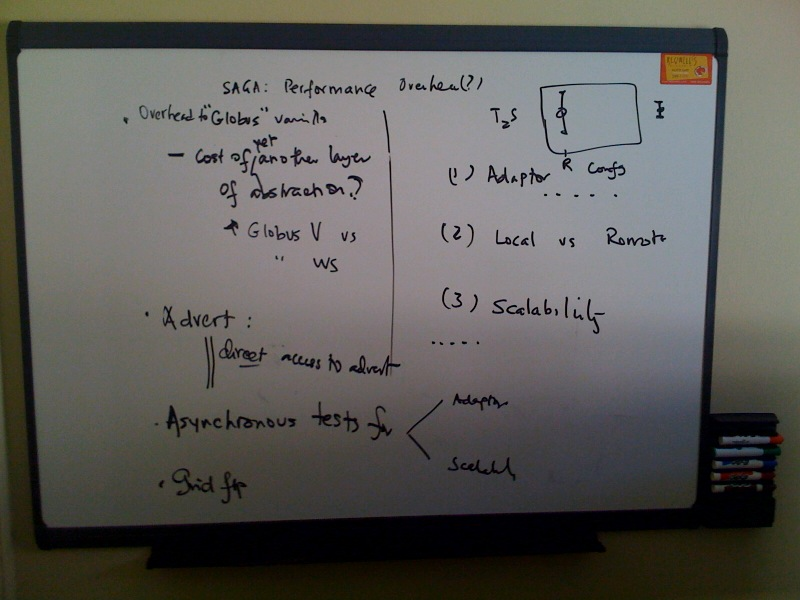
\includegraphics[width=0.65\textwidth]{../figures/ole_board-01.jpg}
 \end{center}
  \up\up\up\up\up\up\up\up\up\up
  \caption{\small Structure of Performance Section..}
 \label{stuff..}
\end{figure}


{\it Deployment and Configuration} Introduce the notion of static
(saga-lite) versus dynamic loading (vanilla saga).

\subsection{Performance}\label{performance}

Although the performance and efficiency of a distributed application mostly depends on the employed programming models and patterns and their suitability for the underlying distributed infrastructure (a choice that can only be made by the developer), SAGA exposes certain performance characteristics and pitfalls that should be taken into consideration when developing distributed applications. Besides a negligible overhead generated by the Engine and its dynamic adaptor loading and selection mechanism (\ref{perf_engine}) SAGA's performance is governed by two major factors: The performance of the middleware adaptor implementations (\ref{perf_adaptors}) and the usage of SAGA's asynchronous interface and task-based operations (\ref{perf_async}). We carried out several benchmarks to pinpoint SAGA’s performance in a production-level environment.   We used an unmodified version of the current SAGA release (1.2.1) on various TeraGrid resources over an extended period of time (to filter out system noise) and where appropriate compared the results to the native middleware tools. In the following, we present our results and discuss their implications for application developers. 

\begin{figure}[!ht]
  \begin{center}
      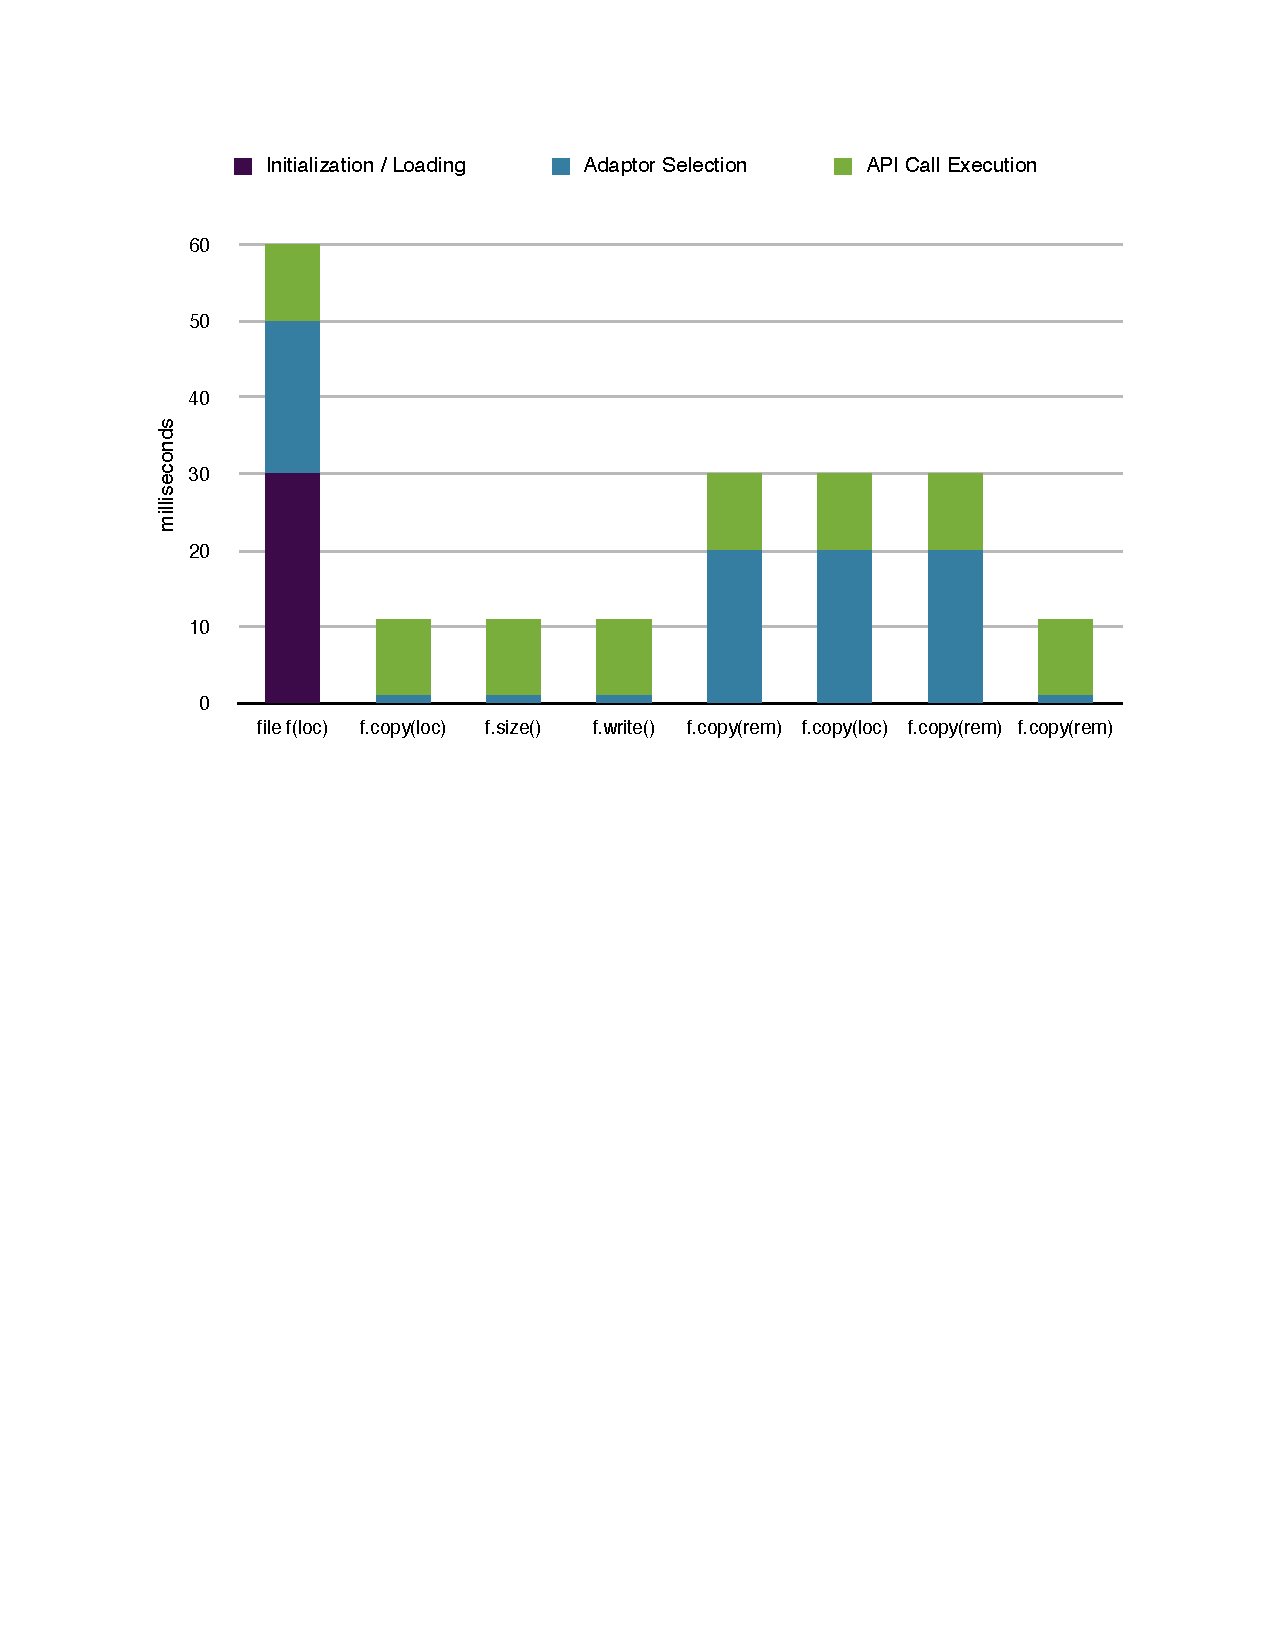
\includegraphics[width=1\textwidth]{../figures/perf_overhead.pdf}
  \end{center}
 \up\up\up\up\up
  \caption{\small SAGA file operations. The first API invocation triggers the initialization and adaptor loading process. The three subsequent calls have virtually no overhead thanks to adaptor priorization. Call 5 to 7 iterate between two different adaptors to execute local (loc) and remote (rem) file copy which causes some adaptor selection overhead.}
 \label{perf_overhead}
\end{figure}

\subsubsection{Engine Performance}\label{perf_engine}
The selection of suitable adaptors to execute an API call at runtime is one of the key features of our C++ SAGA implementation. Naturally, it comes with a certain overhead since it involves several logical steps as depicted in Figure (1). On startup, the Engine parses its configuration file (saga.ini), loads all configured middleware adaptors (dynamic libraries) and registers their capabilities in an internal data structure. The overhead generated by this step varies with the number of configured adaptors but lies generally in the range of 30 milliseconds on an average system. 
If an API method is to be executed, the Adaptor Selector searches the internal adaptor registry for all Adaptors that could potentially execute the API call and tests them one by one.

Our experience with SAGA-based application shows that there’s a high probability that the same adaptor will be selected for many subsequent API calls. In fact, most applications use only one specific middleware Adaptor throughout their entire lifetime. The Engine addresses this by putting the adaptor that executed the last API call in the first position of the registry. This completely eliminates potential adaptor selection overhead for subsequent calls as depicted in Figure \ref{perf_overhead}. But even if this mechanism doesn't kick in due to frequent adaptor changes, the overhead exposed by the adaptor selection is in the order of 20 milliseconds which lies several orders of magnitudes below the typical latencies of a distributed application.


\subsubsection{Adaptor Performance}\label{perf_adaptors}

\subsubsection{Asynchronous Performance}\label{perf_async}


\begin{figure}[!ht]
  \begin{center}
      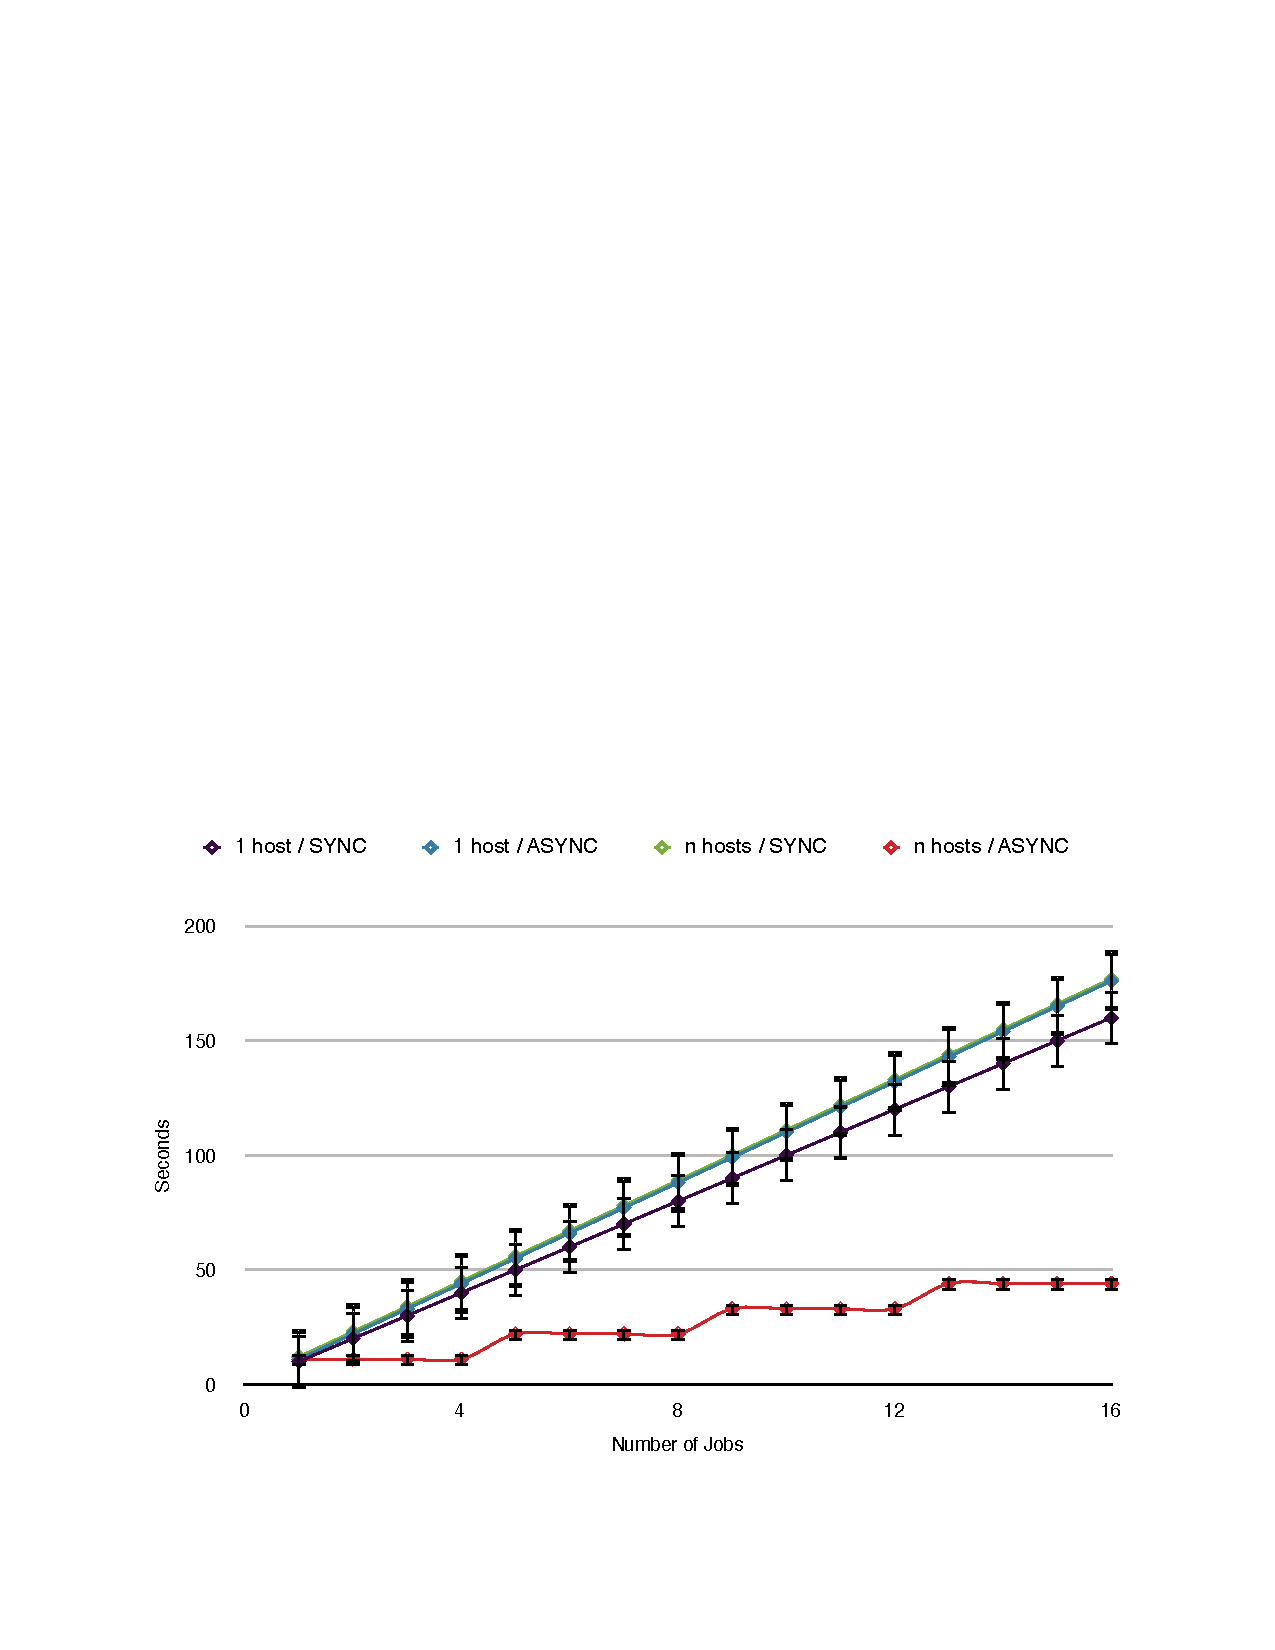
\includegraphics[width=1\textwidth]{../figures/perf_async_1.pdf}
  \end{center}
 \up\up\up\up\up
  \caption{\small Description}
 \label{perf_overhead}
\end{figure}


\section{Applications Redux}{\bf SJ with HK and AM}

\subsection{Closing the Loop}

Show how SAGA helps the problems outlined in Section\ref{application}

\subsection{Discuss Applications Further} {\bf SJ}
 
The Kind of Applications that can be developed..

\section{RoadMap} \note{SJ, AM, HK}

\subsection*{Roadmap from an implementation point of view}
\begin{itemize}
\item CPI for adaptors
\item Upcoming package extension
\item Frameworks/patterns/
\item Other extensions and generalizations
\end{itemize}

\subsection*{Roadmap from a standardization point of view}

\begin{itemize}
\item Packages.. 
\item Functionality
\end{itemize}

\subsection*{Roadmap: Ready for the Next-generation Distributed Application}

\section*{Acknowledgements}


%\bibliographystyle{unsrt}
\bibliographystyle{phcpc}
\bibliography{saga_cpc}
\end{document}
